\documentclass[12pt,a4paper]{article}
\usepackage{../.tex/mcs-notes}
\usepackage{todonotes}

\settitle
{Дискретная математика.}
{\href{mailto:alextiskin@gmail.com}{А. В. Тискин}}
{\%D0\%94\%D0\%B8\%D1\%81\%D0\%9C\%D0\%B0\%D1\%82/DM.pdf}
\date{}

\newcommand{\BB}[1][]{\ensuremath{\mathbb{B}#1}\xspace}

\begin{document}
    \maketitle

    \listoftodos[TODOs]

    \tableofcontents

    \section{Булевые функции}

    \begin{definition}
        $\BB := \{0; 1\}$. \emph{Булевая функция} --- $f: \BB^n \to \BB$.\\
        Множество булевых функций --- $P_2$.\\
        Множество булевых функция --- $P^{(n)}_2$.\\
        Количество всех булевых функция --- $\left|P^{(n)}_2\right|=2^{2^n}$.
    \end{definition}

    \begin{definition}
        Базовые функции:
        \begin{itemize}
            \item $0$, $1$ --- функции-константы.
            \item $\neg x := 1-x$
            \item $\wedge$ и $\vee$ --- стандартные AND и OR. 
        \end{itemize}
    \end{definition}

    \begin{definition}
        Булевая функция $f(x_1, \dots, x_i, \dots, x_n)$ \emph{существенно зависит} от $x_i$, если существуют $a_1, \dots, a_{i-1}, a_{i+1}, \dots, a_n$, что $f(a_1, \dots, a_{i-1}, 0, a_{i+1}, \dots, a_n) \neq f(a_1, \dots, a_{i-1}, 1, a_{i+1}, \dots, a_n)$.
    \end{definition}

    \begin{definition}
        Пусть $F$ --- множество булевых функций. Тогда \emph{сигнатурой $F$} или \emph{множеством формул над $F$} называется множество итеративно заданных формул по принципу:
        \begin{itemize}
            \item формальный символ $x$;
            \item $f(A_1, \dots, A_n)$, где $f\in F$, а $A_1, \dots, A_n$ --- уже определённые функции.
        \end{itemize}

        Формула реализует некоторую функцию (не обязательно из $F$). Формулы реализующие одну и ту же функцию называются \emph{эквивалентными}.
    \end{definition}

    \begin{definition}
        Функция $f$ \emph{выразима} через $F$, если существует формула над $F$, реализующая~$f$.
    \end{definition}

    \begin{definition}
        Замыкание $F$ --- множество $[F]$ функций, выразимых через $F$. 
    \end{definition}

    \begin{statement}\ 
        \begin{itemize}
            \item $F \subseteq [F]$
            \item $F_1 \subseteq F_2 \Rightarrow [F_1] \subseteq [F_2]$
            \item $[[F]] = [F]$
        \end{itemize}
    \end{statement}

    \begin{definition}
        Множество $F$ булевых функций называется \emph{замкнутым}, если $F = [F]$.
    \end{definition}

    \begin{definition}
        Пусть $R$ замкнуто, а $Q\subseteq R$.
        \begin{itemize}
            \item $Q$ \emph{полно для} $R$, если $[Q] = R$.
            \item $R$ \emph{конечно порождаемо}, если существует конечное полное для $R$ множество $Q$, подмножество $R$. Минимальное по включение $Q$ --- \emph{базис} $R$.
        \end{itemize}
    \end{definition}

    \begin{definition}
        Функция $f$ называется монотонной, если \[\forall x_1 \leqslant x'_1, \dots, x_n \leqslant x'_n : f(x_1, \dots, x_n) \leqslant f(x'_1, \dots, x'_n).\]
    \end{definition}

    \begin{statement}
        Множество монотонных функций замкнуто.
    \end{statement}

    \begin{definition}\ \\
        \emph{Литерал} --- это $x$ или $\neg x$, где $x$ --- формальный символ (переменная).\\
        \emph{Элементарная конъюнкция} --- $Y_1 \wedge \dots \wedge Y_k$, где $Y_1, \dots, Y_k$ --- литералы (с попарно различными элементами).\\
        \emph{Элементарная дизъюнкция} --- $Y_1 \vee \dots \vee Y_k$, где $Y_1, \dots, Y_k$ --- литералы (с попарно различными элементами).\\
        \emph{Дизъюнктивная нормальная форма (ДНФ)} --- $Z_1 \vee \dots \vee Z_m$, где $Z_1, \dots, Z_m$ --- (различные) элементарные конъюнкции.\\
        \emph{Конъюнктивная нормальная форма (КНФ)} --- $Z_1 \wedge \dots \wedge Z_m$, где $Z_1, \dots, Z_m$ --- (различные) элементарные дизъюнкции.\\
        \emph{Совершенная ДНФ (СДНФ)} функции $f$ от $n$ переменных --- \[f(x_1, \dots, x_n)=\bigvee_{f(\sigma_1, \dots, \sigma_n)=1} x_1^{\sigma_1} \wedge \dots \wedge x_n^{\sigma_n},\]
        где $x^0 = \neg x$, а $x^1 = x$.\\
        \emph{Совершенная КНФ (СКНФ)} функции $f$ от $n$ переменных --- \[f(x_1, \dots, x_n)=\bigwedge_{f(\sigma_1, \dots, \sigma_n)=0} x_1^{1-\sigma_1} \vee \dots \vee x_n^{1-\sigma_n},\]
        где $x^0 = \neg x$, а $x^1 = x$.
    \end{definition}

    \begin{statement}
        Система $\{\neg, \wedge, \vee\}$ полна (в $P_2$).
    \end{statement}

    \begin{corollary}
        Системы $\{\neg. \wedge\}$, $\{\neg, \vee\}$, $\{1, \wedge, \oplus\}$, $\{\uparrow\}$ и $\{\downarrow\}$ полны.
    \end{corollary}

    \begin{definition}
        Аналогично определяется \emph{(совершенная) конъюктивная нормальная форма (КНФ)}.
    \end{definition}

    \begin{definition}
        \emph{Двойственная функция} к $f$ --- $f^* := \neg f(\neg x_1, \dots, \neg x_n)$.
    \end{definition}

    Свойства:
    \begin{itemize}
        \item $f^{**} = f$
    \end{itemize}

    \begin{statement}[принцип двойственности]
        Если $f$ реализуема формулой $\Phi$, то $f^*$ реализуема формулой $\Phi^*$, где все функции заменяются на двойственные.
    \end{statement}

    \begin{definition}[полином Жегалкина (над $\FF_2$)]
        Выражение функции в базисе $\{1, \wedge, \oplus\}$.
        \[
            f(x_1, \dots, x_n) = \sum_{\{i_1, \dots, i_s\}\subseteq\{1, \dots, n\}} a_{i_1, \dots, i_n} x_{i_1} \dots x_{i_s}
        \]
    \end{definition}

    \begin{theorem}[Жегалкин]
        Любая функция реализуется полиномом Жегалкина единственным образом (с точностью до пропуска членов тождественно равных 0 и перестановок слагаемых и сомножителей). 
    \end{theorem}

    \begin{proof}
        Всего коэффициентов $a_{i_1, \dots, i_s}$ --- $2^n$. Тогда многочленов Жегалкина ровно $2^{2^n}$; сколько и булевых функций. Покажем, что для каждой функций найдётся полином Жегалкина, и тогда докажем теорему.

        Построение полинома аналогично рассуждению в формуле включений-исключений. Сначала рассмотрим значение $f$ в точке $(0, \dots, 0)$: оно определяет свободный член полинома. Далее рассмотрим значение $f$ и имеющегося полинома (пока что состоящего только из, может быть, свободного члена) в точках вида $(0, \dots, 0, 1, 0, \dots, 0)$: по ним определяются коэффициенты при мономах первой степени (по аналогии с формулой включений-исключений). Так далее определяются все коэффициенты.
    \end{proof}

    \begin{definition}
        Функция $f$ \emph{самодвойствена}, если $f=f^*$.
    \end{definition}

    \begin{example}\ 
        \begin{itemize}
            \item $e_i$ и $\neg e_i$ для любого $n$ и $i$ самодвойственны;
            \item $\vee$, $\wedge$, $\oplus$, $\rightarrow$, $\leftarrow$, $\uparrow$ и $\downarrow$ не самодвойствены.
        \end{itemize}
    \end{example}

    \begin{statement}
        Класс $S$ самодвойственных функций замкнут.
    \end{statement}

    \begin{definition}
        $f$ \emph{линейна}, если $f(x_1, \dots, x_n) = a_0 \oplus (a_1 \wedge x_1) \oplus \dots \oplus (a_n \wedge x_n)$ для некоторых $a_1, \dots, a_n$.

        Они же представляются как полиномы Жегалкина степени не выше первой.
    \end{definition}

    \begin{statement}
        Класс $L$ линейных функций замкнут.
    \end{statement}

    \begin{theorem}[теорема Поста]
        Система функций полна (в $P_2$) тогда и только тогда, когда она не содержится целиком ни в одном из $T_0$, $T_1$, $S$, $L$ и $M$.
    \end{theorem}

    \begin{proof}
        Пусть даны $f_0 \notin T_0$, $f_1 \notin T_1$, $f_S \notin S$, $f_L \notin L$, $f_M \notin M$.

        Заметим, что $f_0(x, \dots, x) \in \{1. \neg\}$, а $f_1(x, \dots, x) \in \{0, \neg\}$. Тогда либо $0, 1 \in [\{f_0, f_1\}]$, либо $\neg \in [\{f_0, f_1\}]$.

        Заметим, что для некоторых $\sigma_1, \dots, \sigma_n$ имеем $f_S(\sigma_1, \dots, \sigma_n) = f_S(\neg\sigma_1, \dots, \neg\sigma_n)$. Поэтому $f_S(x^\sigma_1, \dots, x^\sigma_n)$ --- константная функция, а тогда она и $\neg f_S(x^\sigma_1, \dots, x^\sigma_n)$ вместе дают $0$ и $1$, поэтому $0, 1 \in [\{\neg, f_S\}]$.

        Заметим, что $\neg \in [\{0, 1, f_M\}]$.

        Заметим, что $\wedge \in [\{f_L\}]$ или $\uparrow \in [\{f_L\}]$. Для заметим, что в полиноме Жегалкина $f_L$ есть член хотя бы второй степени.
    \end{proof}

    \section{Комбинаторика}

    \subsection{Основы}

    \begin{statement}[правило произведения]
        Если объект $A$ можно выбрать $m$ способами, а $B$ --- $n$, то пару $(A;B)$ можно выбрать $mn$ способами.
    \end{statement}

    \begin{statement}[правило суммы]
        Если объект $A$ можно выбрать $m$ способами, а $B$ --- $n$ способами, то объект ``$A$ или $B$'' --- $m+n$ способами.
    \end{statement}

    \begin{statement}[принцип Дирихле]
        Пусть имеется $n+1$ шаров, разложенных по $n$ урнам, то найдётся урна с хотя бы $2$ шарами.
    \end{statement}

    \begin{statement}[обобщённый принцип Дирихле]
        Пусть имеется $n$ шаров, разложенных по $k$ урнам, то найдётся урна с хотя бы $\lceil\frac{n}{k}\rceil$ шарами.
    \end{statement}

    \subsection{Расстановки и выборки}

    \begin{definition}
        \emph{Упорядоченная расстановка} $n$ элементов в ряд есть упорядоченная последовательность этих $n$ элементов без повторений. Количество упорядоченных расстановок на $n$ элементах равно $n! := \prod_{k=1}^n k$.
        
        \emph{Упорядоченная расстановка} $k$ элементов из $n$ в ряд есть упорядоченная последовательность каких-то $k$ элементов из $n$ без повторений. Количество упорядоченных расстановок $k$ элементов из $n$ равно $P(n, k) = A_n^k = \frac{n!}{(n-k)!}$.

        $k$-элементная \emph{выборка} среди $n$ элементов есть подмножество множества данных $n$ элементов. Таких выборок $\binom{n}{k}=C_n^k = \frac{n!}{k!(n-k)!}$.
    \end{definition}

    \begin{statement}Свойства:
        \begin{enumerate}
            \item $\binom{n}{k}=\binom{n}{n-k}$.
            \item (тождество Паскаля) $\binom{n+1}{k+1} = \binom{n}{k} + \binom{n}{k+1}$.
            \item (биномиальная теорема) \[(x+y)^n=\sum_{k=0}^n \binom{n}{k} x^k y^{n-k}\]
            \item \[\sum_{k=0}^n \binom{n}{k} = 2^n\]
            \item \[\sum_{k=0}^{\lfloor\frac{n}{2}\rfloor} \binom{n}{2k} = 2^{n-1}\]
            \item (тождество Вандермонда) \[\binom{m+n}{k} = \sum_{r=0}^k \binom{m}{r}\binom{n}{k-r}\]
        \end{enumerate}
    \end{statement}

    \begin{definition}
        \emph{Треугольником Паскаля} называется диаграмма следующего вида.

        \[
            \setcounter{MaxMatrixCols}{15}
            \begin{matrix}
                &&&&& 1\\
                &&&& 1 && 1\\
                &&& 1 && 2 && 1\\
                && 1 && 3 && 3 && 1\\
                & 1 && 4 && 6 && 4 && 1\\
                1 && 5 && 10 && 10 && 5 && 1\\
            \end{matrix}
        \]

        Здесь каждое число равно сумме своих верхних соседей, а порождающими являются единичные левая и правая ``стороны'' диаграммы.
    \end{definition}

    Важным замечанием является равенство каждого числа в треугольнике количеству способов добраться до него из верхней единицы, двигаясь только вниз-вправо или вниз-влево. Тем самым $n$-ая строка состоит из чисел $\binom{n}{0}$, $\binom{n}{1}$, \dots, $\binom{n}{n}$.

    В другой интерпретации количество способов добраться из $(0, 0)$ до $(n, m)$, каждый раз увеличивая ровно одну координату на $1$, есть $\binom{n+m}{n}$.
    
    \begin{theorem}[формула Стирлинга]
        $n! \approx \sqrt{2\pi n}(n/e)^n$
    \end{theorem}

    \subsection{Числа Каталана}

    \begin{definition}
        \emph{Правильная скобочная последовательность (ПСП)} --- набор строк, рекуррентно заданных так:
        \begin{itemize}
            \item пустая строка;
            \item если $u$ --- ПСП, то $(u)$ --- ПСП;
            \item если $u$ и $v$ --- ПСП, то $uv$ --- ПСП.
        \end{itemize}

        Множество таких строк называется \emph{языком Дика}.
    \end{definition}

    \begin{definition}
        \emph{Число Каталана $C_n$} --- количество строк Дика длины $2n$.

        \begin{table*}[h]
            \centering
            \begin{tabular}{c|ccccccccc}
                $n$& $0$& $1$& $2$& $3$& $4$& $5$& $6$& $7$& $8$\\
                \hline
                $C_n$& $1$& $1$& $2$& $5$& $14$& $42$& $132$& $429$& $1430$
            \end{tabular}
        \end{table*}
    \end{definition}

    \begin{statement}
        Числа Каталана можно определить рекуррентно:
        \begin{align*}
            C_0 &= 1&
            C_n = \sum_{k=0}^{n-1}C_k C_{n-1-k}
        \end{align*}
    \end{statement}

    \begin{proof}
        ПСП длины $2n > 0$ имеет вид $(S)T$, где для некоторого $k$ $S$ имеет длину $2k$, а $T$ --- $2(n-k-1)$. При фиксированном $k$ количество таких последовательностей равно $C_k C_{n-k-1}$, откуда следует рекурента.
    \end{proof}

    \begin{remark}
        $C_n$ --- количество способов добраться от $(0, 0)$ до $(n, n)$, не выходя выше прямой $x=y$.
    \end{remark}

    \begin{theorem}
        $C_n = \binom{2n}{n} - \binom{2n}{n-1} = \frac{1}{n+1}\binom{2n}{n}$.
    \end{theorem}

    \begin{proof}
        $C_n$ равно количеству способов добраться из $(0, 0)$ до $(n, n)$ не выходя выше прямой $x=y$. Тем самым оно равно количеству всех способов добраться из $(0, 0)$ до $(n, n)$ минус количество способов добраться из $(0, 0)$ до $(n, n)$, пересекая прямую $x+1=y$.

        В каждом из способов дойти от $(0, 0)$ до $(n, n)$, пересекаясь с прямой $x+1=y$, отразим начало пути до первой вершины лежащей на прямой $x+1=y$ относительно данной прямой. Получим биекцию с путями из $(-1, 1)$ в $(n, n)$.

        Отсюда и получаем равенство $C_n = \binom{2n}{n} - \binom{2n}{n+1}$. Вторая часть теоремы выводится несложно алгебраически.
    \end{proof}

    \begin{statement}
        \[C_n \approx \frac{4^n}{n^{3/2}\sqrt{\pi}}\]
    \end{statement}

    \begin{proof}
        По формуле Стирлинга
        \[
            C_n = \frac{1}{(n+1)}\binom{2n}{n} = \frac{(2n)!}{(n!)^2(n+1)} \approx \frac{\sqrt{2\pi 2n}(2n/e)^{2n}}{(2\pi n)(n/e)^{2n}n} = \frac{2^{2n}}{n^{3/2}\sqrt{\pi}} = \frac{4^n}{n^{3/2}\sqrt{\pi}}
        \]
    \end{proof}

    \begin{remark}
        Числа Каталана являются решением для более 30 различных задач. Среди них:
        \begin{itemize}
            \item количество триангуляций правильного $(n+2)$-угольника;
            \item количество способов соединения $2n$ различных точек на окружности $n$ непересекающимися хордами;
            \item количество таблиц Юнга $2 \times n$;
            \item количество бинарных деревьев с $n$ вершинами;
            \item количество плоских деревьев с $n+1$ вершинами;
            \item количество ``фонтанов'' с основанием из $n$ монет;
            \item количество 213-избегающих перестановок длины $n$ (``перестановки, сортируемые при помощи стека'').
        \end{itemize}
    \end{remark}

    \subsection{Производящие функции}

    \begin{definition}
        Производящим рядом последовательности $\{a_i\}_{i=0}^\infty$ является формальный ряд
        \[a_0 + a_1 x + \dots + a_i x^i + \dots = \sum_{i=0}^\infty a_i x^i\]

        Важно понимать, что иногда этот ряд сходится, иногда --- нет. Когда ряд сходится для хотя бы некоторых $x$, её тоже называют производящей функцией данного ряда.
    \end{definition}

    \begin{example}
        Производящие функции простых последовательностей:
        \begin{itemize}
            \item $(1, 1, \dots)$ --- $\frac{1}{1-x}$;
            \item $(\underbrace{1, \dots, 1}_{n+1}, 0, 0, \dots)$ --- $\frac{1-x^n}{1-x}$;
            \item $\{\binom{n}{i}\}_{i=0}^\infty$ --- $(1+x)^n$;
            \item $\{\frac{1}{i!}\}_{i=0}^\infty$ --- $\exp$;
            \item $(0, \frac{1}{1}, \frac{-1}{2}, \frac{1}{3}, \frac{-1}{4}, \dots)$ --- $\ln(1+x)$.
        \end{itemize}
    \end{example}

    \begin{definition}
        Сложение и умножение формальных степенных рядов устроенно следующим образом.
        \begin{itemize}
            \item $\sum_{i=0}^\infty a_i x^i + \sum_{i=0}^\infty b_i x^i = \sum_{i=0}^\infty (a_i + b_i) x^i$
            \item $(\sum_{i=0}^\infty a_i x^i) \cdot (\sum_{i=0}^\infty a_i x^i) = \sum_{i=0}^\infty x^i \sum_{t=0}^i a_t b_{i-t}$
        \end{itemize}
    \end{definition}

    \begin{theorem}[из математического анализа]
        Пусть функция $f$ --- производящая функция последовательности $\{a_i\}_{i=0}^\infty$ --- определена в некоторой окрестности точки $x$ (не обязательно только). Тогда функция $g$ --- производящая функция последовательности $\{(i+1)a_{i+1}\}_{i=0}^\infty$ (т.е. ``производная'' предыдущего ряда) --- определена в точке $x$ и равна $f'(x)$.
    \end{theorem}

    \begin{corollary}
        Теперь можно сказать, что производящая функция $\{i+1\}_{i=0}^\infty$ есть
        \[\sum_{i=1}^\infty ix^{i-1} = \sum_{i=0}^\infty (x^i)' = \left(\sum_{i=0}^\infty x^i\right)'=\left(\frac{1}{1-x}\right)'=\frac{1}{(1-x)^2}\]
    \end{corollary}

    \begin{corollary}
        Одно из доказательств тождества Паскаля легко получается из производящих функций.

        Несложно видеть, что производящие функции $\{\binom{n+1}{k}\}_{k=0}^\infty$, $\{\binom{n}{k}\}_{k=0}^\infty$ и $\{\binom{n}{k-1}\}_{k=0}^\infty$ суть $(1+x)^{n+1}$, $(1+x)^n$ и $(1+x)^n x$ соответственно. При этом $(1+x)^n + (1+x)^n x = (1+x)^{n+1}$, откуда следует, что
        \[\binom{n+1}{k} = \binom{n}{k} + \binom{n}{k-1}\]
    \end{corollary}

    \begin{definition}
        \emph{Обобщённым биномиальным коэффициентом} называется выражение ($u \in \RR$, $k \in \NN \cup\{0\}$)
        \[\binom{u}{k} = \frac{u(u-1)\dots(u-k+1)}{k!} = \frac{\prod_{i=0}^{k-1}(u-i)}{k!}\]
    \end{definition}

    \begin{theorem}[обобщённая биномиальная теорема]
        Для любых $u, x \in \RR$, что $|x| < 1$, верно, что
        \[(1+x)^u = \sum_{k=0}^\infty \binom{u}{k} x^k\]
    \end{theorem}

    \begin{statement}
        Производящая функция чисел Каталана равна $\frac{1-\sqrt{1-4x}}{2x}$.
    \end{statement}

    \begin{proof}
        Пусть производящая функция --- $g$. Тогда заметим, что
        \[g(x)^2 = \sum_{n=0}^\infty x^n \sum_{k=0}^n C_k C_{n-k} = \sum_{n=0}^\infty x^n C_{n+1} = \frac{g(x) - C_0}{x} =\frac{g(x) - 1}{x}\]
        Получаем квадратное уравнение на $g$: $xg^2-g+1=0$. Отсюда имеем, что $g(x)=\frac{1\pm\sqrt{1-4x}}{2x}$. Заметим, что $\sqrt{1-4x} = 1 + \dots$, а $x \mid 1\pm\sqrt{1-4x}$, значит правильный знак --- $1-\sqrt{1-4x}$. Отсюда имеем требуемое утверждение.
    \end{proof}

    \begin{corollary}
        \[C_n = [x^n]g(x) = [x^{n+1}] \frac{1-\sqrt{1-4x}}{2}=\frac{-1}{2}[x^{n+1}]\sqrt{1-4x}=\frac{-1}{2}\binom{1/2}{n+1}(-4)^{n+1}\]
        При этом
        \[\binom{1/2}{n+1} = \frac{(1/2)(-1/2)(-3/2)\dots((1-2n)/2)}{(n+1)!} = \frac{(-1)^n}{2^{n+1}(n+1)!} \cdot 1 \cdot 3 \cdot \dots \cdot (2n-1) = \frac{(-1)^n(2n)!}{2^{2n+1}(n+1)!n!}\]
        Тем самым
        \[C_n = \frac{(2n)!}{(n+1)!n!} = \frac{1}{n+1}\binom{2n}{n}\]
    \end{corollary}

    \section{Теория графов}

    \begin{definition}
        \emph{Граф} --- пара $G = (V, E)$, где $V$ --- (конечное) множество вершин, а $E \subseteq V \times V$ --- множество рёбер.
    \end{definition}

    \begin{definition}
        Граф можно задать \emph{матрицей смежности графа}: это такая матрица $A = (a_{i, j})_{i, j=0}^{|V|}$, где
        \[
            a_{i,j} = \begin{cases}
                1& \text{если $(i, j) \in E$}\\
                0& \text{иначе}
            \end{cases}
        \]
    \end{definition}

    \begin{definition}
        Граф называется \emph{неориентированным}, если для любой пары $(i, j)$ из $E$ верно, что $(j, i) \in E$. В ином случае он называется \emph{ориентированным}.

        По умолчанию подразумеваются именно неориентированные графы.
    \end{definition}

    \begin{definition}
        \emph{Мультиграф} --- граф с кратными рёбрами, т.е. в $E$ могут быть повторения, а в матрице смежности стоять любые натуральные числа.
    \end{definition}

    \begin{definition}
        Вершины $u$ и $v$ смежны, если они соединены ребром: $(u, v) \in E$ или $(v, u) \in E$.

        Вершина $u$ и ребро $e$ называются \emph{инцидентными}, если $e = (u, v)$ или $e = (v, u)$ для некоторой вершины $v$.

        Ребро $(u, u)$ для некоторой вершины $u$ называется \emph{петлёй}.

        \emph{Степень вершины $v$ или $\deg(v)$} --- число инцидентных с вершиной $v$ ребёр, где петли считаются дважды. Также можно просто сказать, что это $|\{(v, u) \in E\} \cup \{(u, v) \in E\}|$.

        \emph{Входящая (исходящая) степень вершины $v$ или $\deg^-(v)$ ($\deg^+(v)$)} в орграфе --- число входящих (исходящих) инцидентных рёбер.
    \end{definition}

    \begin{lemma}
        Сумма степеней вершин графа равна удвоенному количеству рёбер в графе:
        \[
            \sum_{v \in V} \deg(v) = 2 |E|
        \]
    \end{lemma}

    \begin{proof}
        Докажем индукцией по $|E|$.

        \textbf{База.} $|E| = 0$. Нет рёбер, все степени равны нулю.

        \textbf{Шаг.} $|E| = n+1$. Уберём ребро. По предположению индукции в новом графе равенство выполняется. По возвращении ребра на место степени на концах ребра увеличатся на $1$, как и $|E|$. Поэтому равенство останется верным.
    \end{proof}

    \begin{corollary}
        В любом графе чётное количество вершин нечётной степени.
    \end{corollary}

    \begin{lemma}
        В ориентированном графе сумма входящих степеней всех вершин равна сумме исходящих степеней всех вершин и равна количеству рёбер.
    \end{lemma}

    \begin{proof}
        Аналогично при удалении любого ребра в графе все три величины уменьшаются ровно на $1$.
    \end{proof}

    \begin{definition}
        Граф $G' = (V', E')$ называется \emph{подграфом} графа $G = (V, E)$, если $V' \subseteq V$ и $E' \subseteq E$.

        Подграф $G'$ называется \emph{индуцированным множеством вершин $V' \subseteq V$}, если $E' = E \cup (V' \times V')$, т.е. ребро в $G'$ присутствует тогда и только тогда, когда оно же присутствует в $G$ и проведено между вершинами множества $V'$.

        Подграф $G'$ --- остовный подграф графа $G$, если $V' = V$.

        Аналогично вводятся определения и для орграфов.
    \end{definition}

    \begin{definition}
        \emph{Путь, соединяющий $v_0$ и $v_n$}, \emph{путь между $v_0$ и $v_n$} или \emph{путь из $v_0$ в $v_n$} --- совокупность последовательности вершин $\{v_i\}_{i=0}^n$ и последовательности рёбер $\{e_i\}_{i=1}^n$, что $\forall i \in [1, n]$ ребро $e_i = (v_{i-1}, v_i)$ и лежит в $E$.

        Путь называется \emph{простым}, если все вершины, входящие в него различны, и \emph{рё\-бер\-но-\-прос\-тым}, если различны все рёбра, входящие в него.

        Аналогично вводятся определения для орграфов.

        Длина пути --- это длина рёберной последовательности в нём.
    \end{definition}

    \begin{definition}
        \emph{Цикл} --- это путь ненулевой длины, где начальная и конечная вершины совпадают.

        Цикл называется \emph{простым}, если его длина хотя бы $3$ и все его вершины кроме последней попарно различны.

        Цикл называется \emph{рёберно-простым}, если его длина хотя бы $3$ и все его рёбра попарно различны.
    \end{definition}

    \begin{definition}
        Если между двумя вершинами неориентированного графа есть путь, то они называются \emph{связанными}. Если граф ориентированный, то две вершины называются \emph{слабо-связанными}, если воспринимать граф как неориентированный и в таком случае они связанные, а также называются \emph{сильно-связанными}, если между ними есть по пути в обе стороны.

        ``Связанность'', ``слабая связанность'' и ``сильная связанность'' -- отношения эквивалентности. Поэтому их классы эквивалентности называют \emph{компонентами связности}, \emph{компонентами слабой связности} и \emph{компонентами сильной связности} соответственно.

        Неориентированный граф, в котором ровно одна компонента связности, называется \emph{связным}. Оргаф, в котором ровно одна компонента слабой (сильной) связности, называется \emph{слабо (сильно) связным}.
    \end{definition}

    \begin{statement}
        Компонента связности (слабой связности / сильной связности) является связным (слабо связным / сильно связным) подграфом.
    \end{statement}

    \begin{remark}
        Между компонентами связности или слабой связности не проходит никаких рёбер.
        
        Между же компонентами сильной связности рёбра проходить могут, но строго в одну сторону (от одной компоненты к другой). В таком случае можно построить орграф, вершинами которого являются компонентами сильной связности изначального графа связности, а ребро от компоненты $A$ к компоненте $B$ будет проведено тогда и только тогда, когда в изначальном графе есть ребро из вершины компоненты $A$ в вершину компоненты $B$. Такой граф называется \emph{граф конденсации (condensation graph)} изначального графа, а процесс его построения называется \emph{конденсацией} изначального графа (\emph{building of condensation graph}).
    \end{remark}

    \begin{exercise*}
        Докажите, что на вершинах графа конденсации можно ввести линейный порядок $\preccurlyeq$, что если присутствует ребро $(u, v)$, то $u \succcurlyeq v$.
    \end{exercise*}

    \begin{definition}
        \emph{Эйлеров путь (цикл)} --- рёберно-простой путь (цикл), содержащий все рёбра графа.
    \end{definition}

    \begin{theorem}[Эйлера]\ 
        \begin{enumerate}
            \item Связный граф имеет эйлеров цикл тогда и только тогда, когда все вершины в нём чётной степени.
            \item Связный граф имеет эйлеров путь тогда и только тогда, когда все вершины в нём кроме либо ровно двух вершин, либо ни одной чётной степени.
        \end{enumerate}
    \end{theorem}
    
    \begin{proof}
        \begin{enumerate}
            \item
                Каждый раз, когда та или иная вершина упоминается в рёберно-простом пути, используется два инцидентных с этой вершиной ребра, значит у каждой вершины используется чётное число рёбер. В таком случае, если эйлеров цикл есть, то у каждой вершины чётная степень.
    
                Пусть у каждой вершины чётная степень. Выйдем из случайной вершины и будем идти по рёбрам, по которым раньше не ходили, пока не вернёмся в какую-либо вершину, в которой уже были. Оторвав начало нашего пути до данной вершины, получим рёберно-простой цикл. Убрав все его рёбра из графа получим граф, в котором все степени вершин чётны (но граф уже не обязательно связен). Повторив операцию ещё несколько раз, получим представление множества рёбер в виде дизъюнктного объединения рёберно-простых циклов. Возьмём любые два из этих цикла, имеющих общую вершину и объединим их в один (новый цикл будет выглядеть как сначала обход первого цикла от нашей вершины, а потом второго). Представление в виде дизъюнктного объединения не исчезнет, поэтому будем делать эту операцию, пока можем. В конце получаем циклы, которые даже вершинами не пересекаются. Поскольку граф связен, то таких циклов, значит он и является искомым эйлеровым.
            \item
                Если есть эйлеров путь, который не цикл, то можно в граф добавить вершину, соединённую ровно с началом и концом пути. В таком случае получим эйлеров цикл, а значит степени всех вершин чётны. Убрав вершину обратно, получим, что у ровно только у концов эйлерова пути поменялась чётность степени, значит вершин нечётной степени ровно две.

                Если степени всех вершин чётные, то в графе есть 
        \end{enumerate}
    \end{proof}

    \begin{theorem}[Эйлера, ориентированная]\ 
        \begin{enumerate}
            \item Связный орграф имеет эйлеров цикл тогда и только тогда, когда каждая вершина в нём имеет равные входящую и исходящую степени.
            \item Связный орграф имеет эйлеров путь тогда и только тогда, когда каждая вершина в нём кроме, быть может, ровно двух имеет равные входящую и исходящую степени. При этом из двух исключенных вершин, если они имеются, одна имеет входящую степень на 1 больше исходящей, а вторая имеет исходящую степень на 1 больше входящей.
        \end{enumerate}
    \end{theorem}

    \begin{proof}
        Абослютно аналогично неориентированному случаю.
    \end{proof}

    \begin{definition}
        Пусть дан $k$-символьный алфавит $\Sigma$. Тогда \emph{граф де Брейна} порядка $n$ --- граф построенный по следующим условиям:
        \begin{enumerate}
            \item множество вершин $V = \Sigma^n$;
            \item из каждой вершин $w_1\dots w_n$ выходит по ориентированному ребру в каждую из вершин $w_2\dots w_n b$, $b \in \Sigma$.
        \end{enumerate}
    \end{definition}

    \begin{remark}
        В графе де Брейна есть Эйлеров цикл. Действительно, из каждой вершины выходит $k$ рёбер (по определению) и входит $k$ рёбер (т.к. все рёбра входят из вершин, получаемых удалением последнего символа и добавлением в начало абсолютно любого символа, т.е. таких вершин тоже $k$).

        При этом каждое ребро эквивалентно некоторой строке длины $n+1$. Таким образом эйлеров цикл эквивалентен слову длины $n + k^{n+1}$, где каждая строка длины $n+1$ встречается как подстрока ровно по разу.
    \end{remark}

    \begin{definition}
        Гамильтонов путь (цикл) --- путь (цикл), проходящий по каждой вершине графа ровно по разу.
    \end{definition}

    \begin{remark}
        В отличие от эйлерова пути, легко проверяемых критериев существования гамильтонова пути или цикла не известно (NP-полная задача, одна из Проблем тысячелетия института Клэя).
    \end{remark}

    \begin{theorem}[Дирака]\label{Dirac's-theorem}
        Если в графе $G$ с $n \geqslant 3$ вершинами сумма степеней любых двух вершин $\geqslant n-1$ (соответственно, $\geqslant n$), в нём существует гамильтонов путь (соответственно, цикл).
    \end{theorem}

    \begin{lemma}
        Если в графе с $k \geqslant 3$ вершинами имеется гамильтонов путь, и сумма степеней этого пути $\geqslant k$, то в нём имеется и гамильтонов цикл.
    \end{lemma}

    \begin{proof}
        Пусть $p = A_1A_2\dots A_k$ --- гамильтонов путь, $\deg(A_1) = l$. Назовём отмеченными вершины, предшествующие (в смысле порядка от $A_1$ до $A_k$) в пути $p$ тем $l$ вершинами, с которыми смежна $A_1$. Заметим, что $\deg(A_k) \geqslant k - \deg(A_1) = k - l$, следовательно по принципу Дирихле будет отмеченная вершина, смежная с $A_k$; пусть это будет $A_i$. Тогда существует гамильтонов цикл $A_1 A_2\dots A_i A_k A_{k-1} \dots A_{i+1} A_i$.
    \end{proof}

    \begin{varproof}{Доказательство \hyperref[Dirac's-theorem]{теоремы Дирака}}
        По лемме, достаточно доказать, что для пути. Пусть $p$ --- самый длинный простой путь. Предположим, что он содержит $k < n$ вершин.

        Заметим, что если $n > 3$, то $n - 1 \geqslant 3$, а значит есть вершина степени $\geqslant 2$, а тогда есть простой путь длины $3$, и тогда $k \geqslant 3$. Если $n = 3$, то среди трёх возможных рёбер графа может отсутствовать не более одного (иначе степени будут равны $0$, $\leqslant 1$ и $\leqslant 1$, и тогда условие, что сумма степеней любых двух вершин $\geqslant n - 1 = 2$ не верно). В таком случае точно есть путь длины $3$, следовательно $k \geqslant 3$. Значит в любом случае $k \geqslant 3$.

        Пусть $H$ --- граф, индуцированный вершинами пути $p$. Путь $p$ является гамильтоновым в $H$. Концы пути $p$ соединены только с другими вершинами $p$, так как иначе $p$ продлевается в $G$. В таком случае у концов пути сумма степеней не менее $n - 1 \geqslant k$, а значит применима лемма. Тогда получаем, что в $G$ есть простой цикл $p$ длины $k$.
        
        Цикл $p$ не соединён с вершинами вне него, так как иначе его можно превратить в путь длины $k + 1$. Значит степени всех вершин цикла $\leqslant k - 1$, а степени остальных вершин $\leqslant n - k - 1$. Если существуют вершины обоих типов, то беря вершину из цикла и вершину вне него, имеем, что сумма их степеней равна $n - k - 1 + (k - 1)= n - 2 < n - 1$ --- противоречие с условием. Следовательно либо $k = 0$, что очевидно неверно, либо $k = n$. Таким образом в $G$ есть гамильтонов путь.
    \end{varproof}

    \begin{definition}
        \emph{Лес (ациклический граф)} --- граф без простых циклов.

        \emph{Дерево} --- связный лес.

        \emph{Ориентированное дерево} --- орграф без циклов, в котором одна вершина имеет входящую степень $0$, а все остальные вершины имеют входящую степень $1$. \emph{Корень} ориентированного дерева --- вершина с входящей степенью $0$, а \emph{лист} ориентированного дерева --- вершина с исходящей степенью $0$.
    \end{definition}

    \begin{definition}
        \emph{Мост} --- ребро, удаление которого увеличивает число компонент связности.
    \end{definition}

    \begin{theorem}[о мостах]
        Ребро является мостом тогда и только тогда, когда не принадлежит ни одному простому циклу.
    \end{theorem}

    \begin{proof}
        Пусть $G = (V, E)$, $e \in E$; обозначим $G \setminus e = (V, E \setminus \{e\})$.

        Если ребро $e$ содержится в простом цикле $e, e_1, e_2, \dots, e_k$, то для всякого пути $g_1, \dots, g_n$ можно заменить все вхождения $e$ на $e_1, \dots, e_k$ (или развёрнутый путь, если проход по $e$ был в обратную сторону), получив путь с теми же концами, но без ребра $e$. Поэтому если две какие-то вершины связаны в $G$, то связаны и в $G \setminus e$. Поэтому $e$ не мост.

        Если ребро $e$ не содержится в простых циклах в $G$, то нет простого пути в $G \setminus e$, соединяющего концы ребра $e$, так как иначе его можно дополнить ребром $e$ до простого цикла в $G$, а значит нет никаких путей в $G \setminus e$ между концами $e$, значит они стали находится в разных компонентах связности. Тогда понятно, что количество компонент связности увеличилось. Таким образом $e$ --- мост.
    \end{proof}

    \begin{definition}
        \emph{Простой граф} --- неориентированный граф без петель и кратных рёбер.
    \end{definition}

    \begin{theorem}[о деревьях]
        Для простого графа $G$ следующие утверждения равносильны:
        \begin{enumerate}
            \renewcommand{\labelenumi}{(\theenumi)}
            \item $G$ --- дерево;
            \item любые две вершины в $G$ соединены ровно одним простым путём;
            \item $G$ ацикличен, но если любую пару несмежных вершин соединить ребром, то в полученном графе образуется ровно один простой цикл;
            \item $G$ связен и $|V| = |E| + 1$;
            \item $G$ ацикличен и $|V| = |E| + 1$;
            \item $G$ связен, и всякое ребро в $G$ является мостом.
        \end{enumerate}
    \end{theorem}

    \begin{proof}
        Будем по очереди показывать равносильность (1) c каждым из (2)-(6).
        \begin{enumerate}
            \setcounter{enumi}{1}
            \renewcommand{\labelenumi}{(\theenumi)}
            \item Пусть $G$ --- дерево. Из-за связности любые две вершины соединены простым путём. Предположим между двумя вершинами есть два простых пути: $v_0 \to \dots \to v_n$ и $u_0 \to \dots \to u_m$, что $v_0 = u_0$, а $v_n = u_m$. Тогда есть такое $i$, что $v_0 = u_0$, $v_1 = u_1$, \dots , $v_i = u_i$, а $v_{i+1} \neq u_{i+1}$. Рассмотрим Минимальное $j > i$, что $v_j$ принадлежит второму пути (такое $j$ точно есть, так как $v_n = u_m$, а значит принадлежит второму пути). Тогда $v_j = u_k$ для некоторого $k$, а цикл $v_i \to v_{i+1} \to \dots \to v_j = u_k \to u_{k-1} \to \dots \to u_i = v_i$ является простым --- противоречие. Значит есть не более одного пути.
            
            Пусть теперь дан граф $G$, что любые две вершины в $G$ соединены ровно одним простым путём. Тогда $G$ связен. А если в $G$ есть простой цикл, то между любыми двумя его различными вершинами есть хотя бы два простых пути, значит $G$ ацикличен. Таким образом $G$ --- дерево.

            \item Пусть $G$ --- дерево. Тогда $G$ ацикличен. При этом между любыми двумя несмежными вершинами есть простой путь, а значит если к нему добавить ребро, соединяющее эти две вершины, то получится простой цикл. При этом два цикла таким образом получится не могут, так как иначе, удалив это ребро, мы получим два простых пути, что не может быть по пункту (2).
            
            Пусть теперь $G$ --- ациклический граф, что если между двумя его несмежными вершинами добавить ребро, то появится ровно один простой цикл. Понятно, что тогда $G$ связен, так как иначе можем соединить две вершины из разных компонент связности, и добавленный мост не должен будет создавать циклы, но создаст. При этом $G$ связен, значит $G$ --- дерево.

            \item Пусть $G$ --- это дерево. Тогда заметим, что либо $|V| = 1$, либо в $G$ есть вершина степени $1$. Действительно, если их нет, то мы можем встать в любую вершину и идти каждый раз по новому ребру, пока не придём в вершину, в которой уже были, и тем самым сделаем простой цикл. Значит висячая вершина есть, а тогда убирая её из графа, мы оставляем $G$ связным и ацикличным, а $|V|$ и $|E|$ уменьшаются ровно на $1$, значит $|V| - |E|$ не меняется. Такими действиями мы дойдём до случая, когда $|V| = 1$, а в таком случае $|E| = 0$, значит $|V| - |E| = 1$ с самого начала. Т.е. $|V| = |E| + 1$. Связность $G$ уже гарантирована.
            
            Пусть $G$ --- связный граф, что $|V| = |E| + 1$. Тогда
            \[\frac{\sum_{v \in V} \deg(v)}{|V|} = \frac{2|E|}{|V|} = 2\frac{|V|-1}{|V|} = 2 - \frac{2}{|V|} < 2\]
            а значит есть вершина степени не более $1$. При этом если есть вершина степени $0$, то $|V| = 1$, поэтому $G$, действительно, дерево. Если же в нём нет вершин степени $0$, то есть висячая. Тогда несложно понять по индукции по $|V|$, что $G$ --- дерево: можно убрать висячую вершину, граф останется связным и с условием $|V| = |E| + 1$, тогда по предположению индукции он --- дерево, а если на него обратно навесить висячую вершину, то он останется деревом.

            \item Пусть $G$ --- дерево. Тогда $G$ по определению ацикличен; а в предыдущем пункте мы показали, что $|V| = |E| + 1$.
            
            Пусть $G$ --- ациклический граф, что $|V| = |E| + 1$. Тогда каждая его компонента связности --- ациклический связный граф, т.е. дерево. Тогда если $V_1$, $V_2$, \dots, $V_n$ --- компоненты связности, а $E_1$, \dots, $E_n$ --- рёбра в них, то для каждой из них верно, что $|V_i| = |E_i| + 1$. Следовательно
            \[|V| = \sum_{i=1}^n |V_i| = \sum_{i=1}^n |E_i| + 1 = |E| + n.\]
            Но тогда $n=1$, значит граф связен, а тогда он --- дерево.

            \item Вспомним, что ребро является мостом тогда и только тогда, когда оно не содержится ни в одном простом цикле графа. Каждое ребро графа является мостом тогда и только тогда, когда в графе нет простых циклов, т.е. он ацикличен. Тогда $G$ связен и каждое его ребро --- мост тогда и только тогда, когда $G$ связен и ацикличен, тогда и только тогда, когда $G$ --- дерево.
        \end{enumerate}
    \end{proof}

    \begin{definition}
        \emph{Остовное дерево} --- остовный подграф, который является деревом.
    \end{definition}

    \begin{lemma}
        Всякий связный граф содержит остовное дерево.
    \end{lemma}

    \begin{proof}
        Если связный граф ацикличен, то он сам является своим остовным деревом.

        Иначе удалим произвольное ребро, входящее в некоторый простой цикл. Граф останется свяным. Так будем делать до тех пор, пока не получим ациклический граф. Тогда получившийся граф окажется остовным деревом изначального графа.
    \end{proof}

    \begin{corollary}
        В связном графе $|E| \geqslant |V| - 1$.
    \end{corollary}

    \begin{definition}
        Графы $G_1 = (V_1, E_1)$ и $G_2 = (V_2, E_2)$ \emph{изоморфны}, если существует биекция $f: V_1 \to V_2$, что для всяких $u, v \in V_1$ верно, что $(u, v) \in E_1 \leftrightarrow (f(u), f(v)) \in E_2$.

        Аналогично для ориентированных графов.
    \end{definition}

    \begin{remark}
        Графы изоморфны тогда и только тогда, когда вершины одного из них можно перенумеровать так, что их матрицы смежности совпадут.
    \end{remark}

    \begin{definition}
        Граф --- \emph{плоский}, если его можно изобразить на плоскости без пересечения рёбер так, что его вершины представлены точками плоскости, а рёбра --- непересекающимися кривыми на ней, соединяющими смежные вершины (\emph{укладка} графа на плоскости).

        Более формально, рёбра достаточно представлять ломанными с конечным числом звеньев.

        Области, на которые укладка графа разбивает плоскость, называются её \emph{гранями}, в том числе и неограниченная область (\emph{внешняя грань}).

        В таком случае $G = (V, E, F)$, где $F$ --- множество граней графа $G$.

        \emph{Планарный граф} --- граф, изоморфный плоскому (т.е. имеющий укладку).
    \end{definition}

    \begin{theorem}
        Граф планарен тогда и только тогда, когда имеет укладку на сфере.
    \end{theorem}

    \begin{proof}
        используя стереографическую проекцию мы можем построить непрерывную биекцию между плоскостью и сферой без точки. Тогда если граф вкладывается в плоскость, то вкладывается и в сферу. При этом выбирая любую точку с любой грани и делая проекцию через неё, получаем из вложения графа в сферу вложение графа в плоскость.
        \begin{figure}[h]
            \centering
            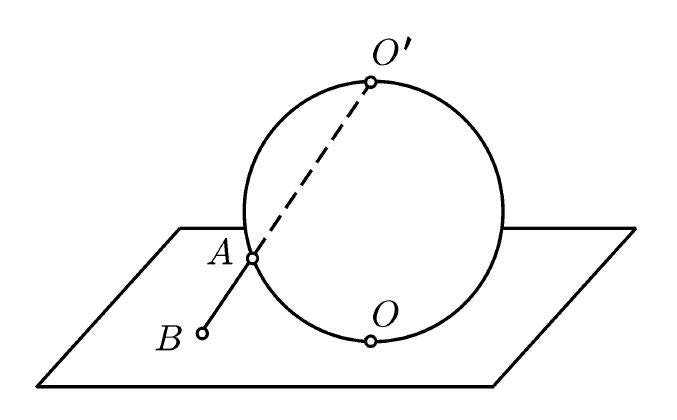
\includegraphics[height=5cm]{DM-01.jpg}
        \end{figure}
    \end{proof}
\end{document}